\documentclass{article}
\usepackage[utf8]{inputenc}
\usepackage{hyperref}
\usepackage{multirow}
\hypersetup{
    colorlinks,
    citecolor=black,
    filecolor=black,
    linkcolor=black,
    urlcolor=black
}
\usepackage{listings}
\usepackage[T1]{fontenc}
\usepackage{xcolor}
\usepackage{textcomp}
\usepackage{graphicx}
%New colors defined below
\definecolor{codegreen}{rgb}{0,0.6,0}
\definecolor{codegray}{rgb}{0.5,0.5,0.5}
\definecolor{codepurple}{rgb}{0.58,0,0.82}
\definecolor{backcolour}{rgb}{0.95,0.95,0.92}
\definecolor{codebg}{HTML}{EEEEEE}
\definecolor{codeframe}{HTML}{CCCCCC}
%Code listing style named "mystyle"
\lstdefinestyle{mystyle}{
  backgroundcolor=\color{backcolour},   commentstyle=\color{codegreen},
  keywordstyle=\color{magenta},
  numberstyle=\tiny\color{codegray},
  stringstyle=\color{codepurple},
  rulecolor=\color{codeframe},
  basicstyle=\ttfamily\footnotesize,
  frame=single,
  framesep=10pt,
  breakatwhitespace=false,
  upquote=true,
  breaklines=true,                 
  captionpos=b,                    
  keepspaces=true,                 
  numbers=none,                    
  numbersep=5pt,                  
  showspaces=false,                
  showstringspaces=false,
  showtabs=false,                  
  tabsize=2,
  columns=flexible
}
\makeatletter
\def\lst@outputspace{{\ifx\lst@bkgcolor\empty\color{white}\else\lst@bkgcolor\fi\lst@visiblespace}}
\makeatother
%"mystyle" code listing set
\lstset{style=mystyle}

\title{Programmes}
\date{ }

\begin{document}
\begin{center}


\rule{\textwidth}{1.6pt}\vspace*{-\baselineskip}\vspace*{2pt} % Thick horizontal line
\rule{\textwidth}{0.4pt}\\[\baselineskip] % Thin horizontal line

{\LARGE Mathematical Physics Lab Practicals \\[0.2\baselineskip] }% Title

\rule{\textwidth}{0.4pt}\vspace*{-\baselineskip}\vspace{3.2pt} % Thin horizontal line
\rule{\textwidth}{1.6pt}\\[2\baselineskip] % Thick horizontal line

\textbf{\Large \\[\baselineskip] SGTB Khalsa College, University of Delhi}\\[\baselineskip]
\textbf{\Large Preetpal Singh(2020PHY1140)}\\[\baselineskip] 

\vspace*{\baselineskip}
\textbf{\Large University Roll No: 20068567043}\\[\baselineskip] 
\vspace*{\baselineskip}
\textbf{\Large Unique Paper Code: 32221301}\\[\baselineskip] 
\vspace*{\baselineskip}
 
\textbf{\Large Paper Title: Mathematical Physics Lab}\\[\baselineskip] 
\vspace*{\baselineskip}
\textbf{\Large \\[\baselineskip] Submitted to: Dr. Savinder Kaur}\\[\baselineskip]
\textbf{\Large Sushil Kumar Singh}\\[\baselineskip]

\end{center}
\newpage

\maketitle
  
\tableofcontents
\begin{table}[]
\begin{tabular}{lrrll}
\textbf{Practical}                                                              & \multicolumn{1}{l}{\textbf{Submission}} & \multicolumn{1}{l}{\textbf{Page No.}} &  &  \\
Trapezoidal and Simpson Method                                         & Sep 20, 2021                           & 4                            &  &  \\
Legendre Polynomial                                                    & Sep 21, 2021                           & 9                            &  &  \\
Lagrange Interpolation                                                 & Sep 27, 2021                           & 16                           &  &  \\
Radioactive Decay, RC Circuit and Stokes Law by Euler, RK2, RK4 Method & Oct 16, 2021                           & 20                           &  &  \\
2nd Order Coupled diffential equations using Euler, RK2, RK4 Method    & Oct 26, 2021                           & 28                           &  &  \\
RK4 Method for Simulataneous Differential Equations                    & Nov 2, 2021                            & 34                           &  &  \\
Gauss Elimination Method                                               & Nov 16, 2021                           & 39                           &  &  \\
Gauss Seidel Method                                                    & Nov 22, 2021                           & 42                           &  & 
\end{tabular}
\end{table}
\clearpage
\begin{figure}[h]
    \centering
    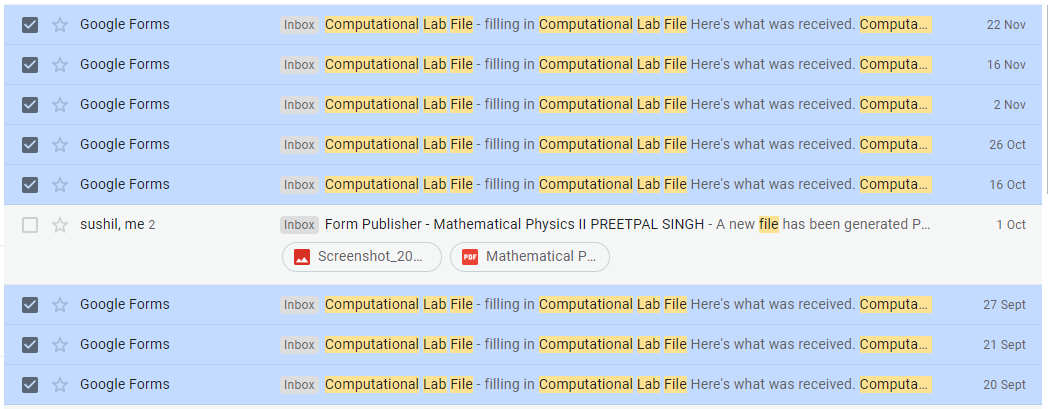
\includegraphics[width=15cm,height=10cm \textwidth]{Capture.PNG}
\caption{Submission of all Practicals}
\end{figure}
\clearpage
\begin{figure}[h]
    \centering
    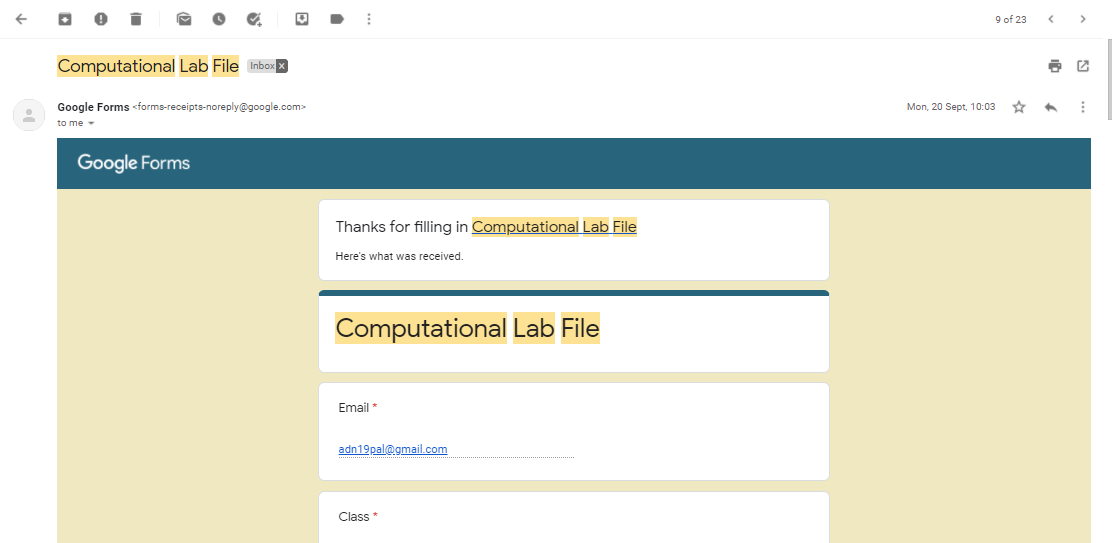
\includegraphics[width=15cm,height=7cm \textwidth]{1.PNG}
\caption{Trapezoidal and Simpson Method}
\end{figure}
\section{Trapezoidal and Simpson Method}
%Importing code from file
%%%%%%%%%%%%%%%%%%%%%%%%%%%%%%%%%%%%%%%%%%%%%%%%%%%%%%%%%%%%%%%%%%%%%
\lstinputlisting[language=python, 
caption=Trapezoidal and Simpson Method
]{Trapezoidal_and_simpson/trep_simp.py}

\newpage
\begin{figure}[h]
    \centering
    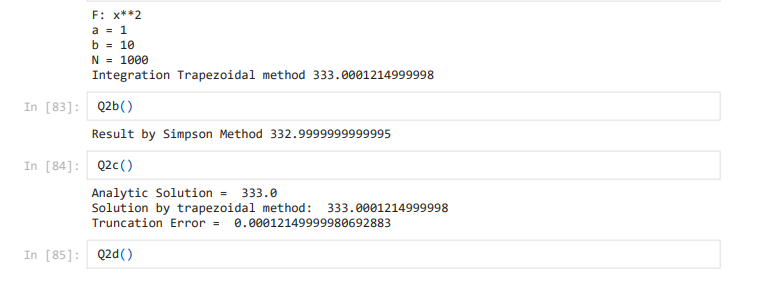
\includegraphics[width=15cm,height=5cm \textwidth]{Trapezoidal_and_simpson/2.PNG}
\caption{Trapezoidal and Simpson Method Output}
\end{figure}
\begin{figure}[h]
    \centering
    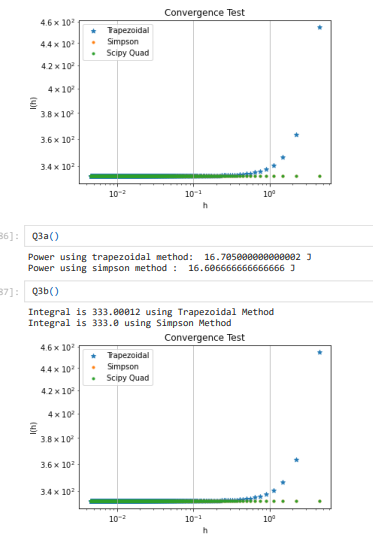
\includegraphics[width=15cm,height=12cm \textwidth]{Trapezoidal_and_simpson/Capture.PNG}
\caption{Trapezoidal and Simpson Method Output}
\end{figure}

%%%%%%%%%%%%%%%%%%%%%%%%%%%%%%%%%%%%%%%%%%%%%%%%%%%%%%%%%%%%%%%%%%%%%
\clearpage
\begin{figure}[h]
    \centering
    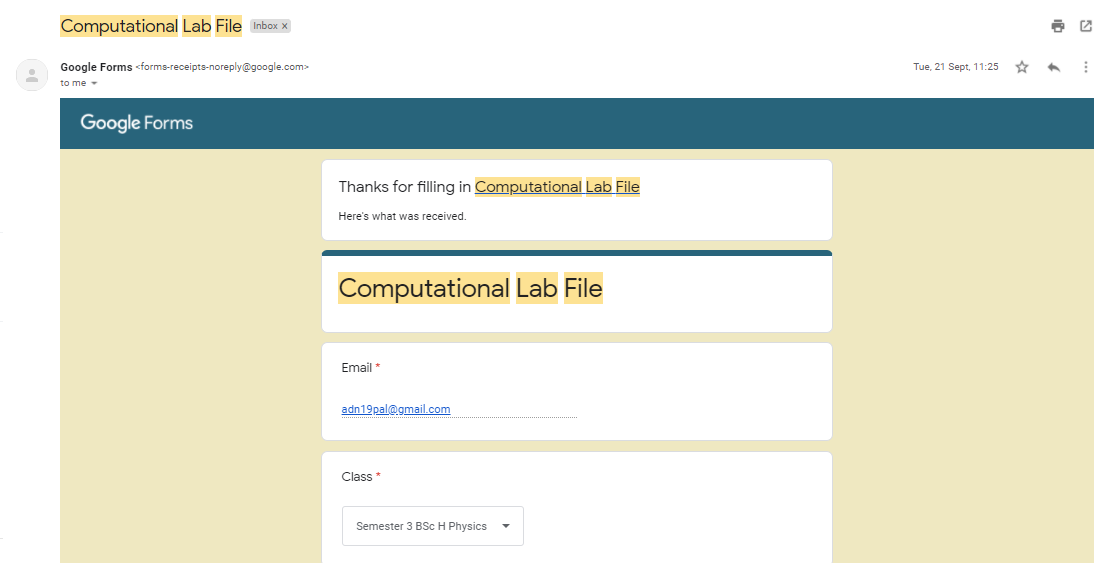
\includegraphics[width=16cm,height=10cm \textwidth]{2.PNG}
\caption{Legendre}
\end{figure}
\section{Legendre Polynomial}
\lstinputlisting[language=python, 
caption=Legendre Polynomial
]{Legendre/Legendre.py}

\begin{figure}[h]
    \centering
    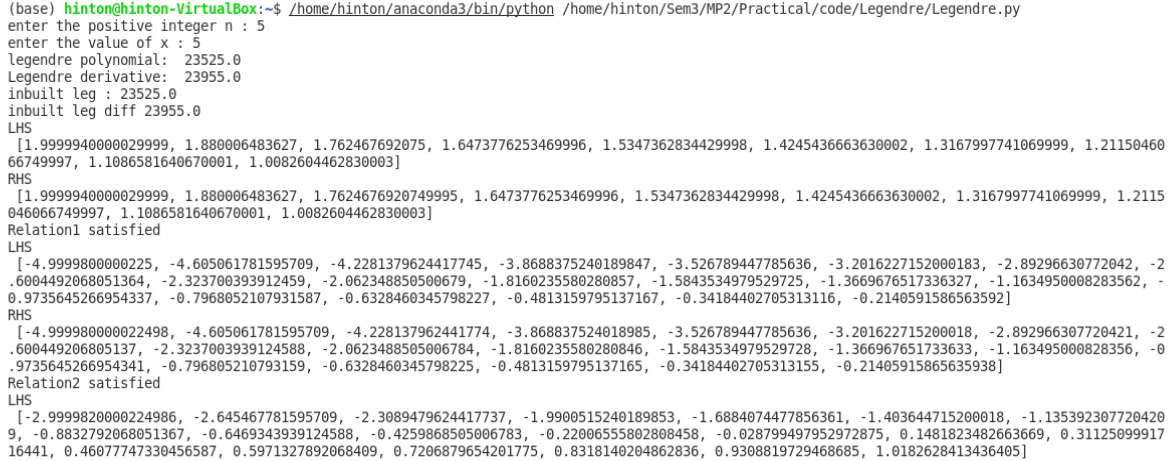
\includegraphics[width=16cm,height=7cm \textwidth]{Legendre/3.PNG}
\caption{Legendre}
\end{figure}
\begin{figure}[h]
    \centering
    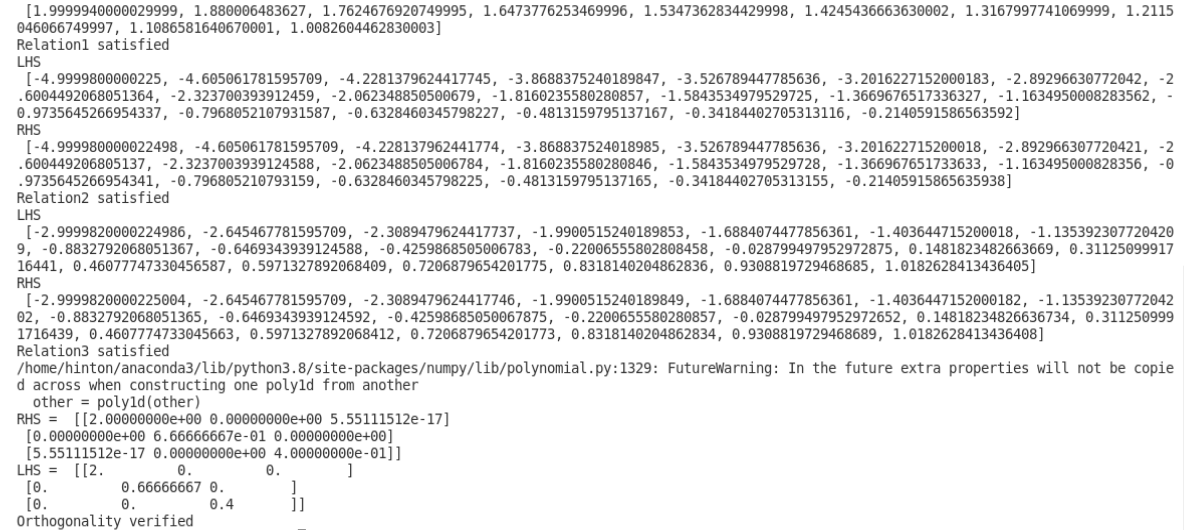
\includegraphics[width=16cm,height=7cm \textwidth]{Legendre/4.PNG}
\caption{Legendre}
\end{figure}
\clearpage
\begin{figure}[h]
    \centering
    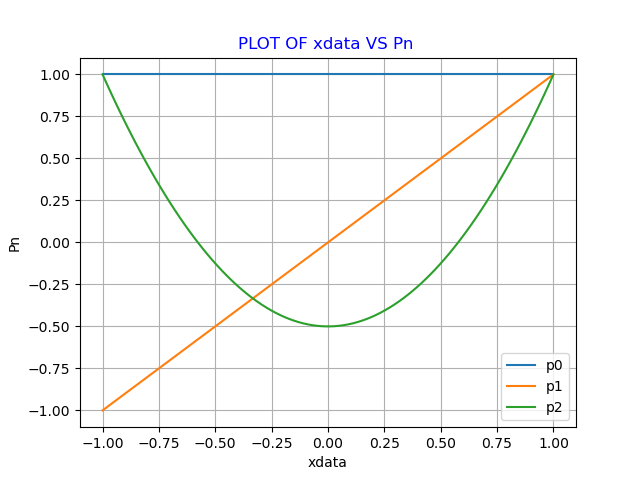
\includegraphics[width=12cm,height=10cm \textwidth]{Legendre/Figure_1.png}
\caption{Legendre}
\end{figure}
\clearpage
\begin{figure}[h]
    \centering
    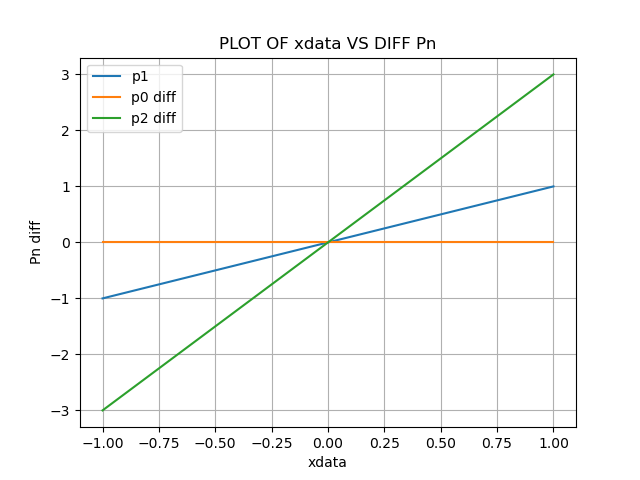
\includegraphics[width=12cm,height=10cm \textwidth]{Legendre/Figure_2.png}
\caption{Legendre}
\end{figure}

%%%%%%%%%%%%%%%%%%%%%%%%%%%%%%%%%%%%%%%%%%%%%%%%%%%%%%%%%%%%%%%%%%%%%
\newpage
\begin{figure}[h]
    \centering
    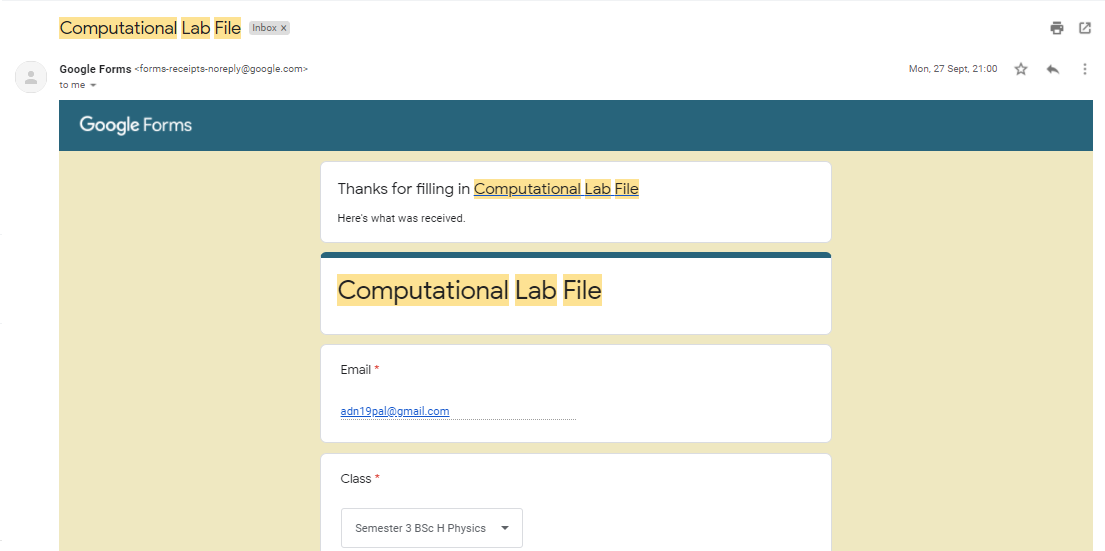
\includegraphics[width=15cm,height=12cm \textwidth]{3.PNG}
\caption{Lagrange Interpolation}
\end{figure}
\section{Lagrange Interpolation}
\lstinputlisting[language=python, 
caption=Lagrange Interpolation
]{Lagrange_Interpolation/Lagrange.py}

\newpage
\begin{figure}[h]
    \centering
    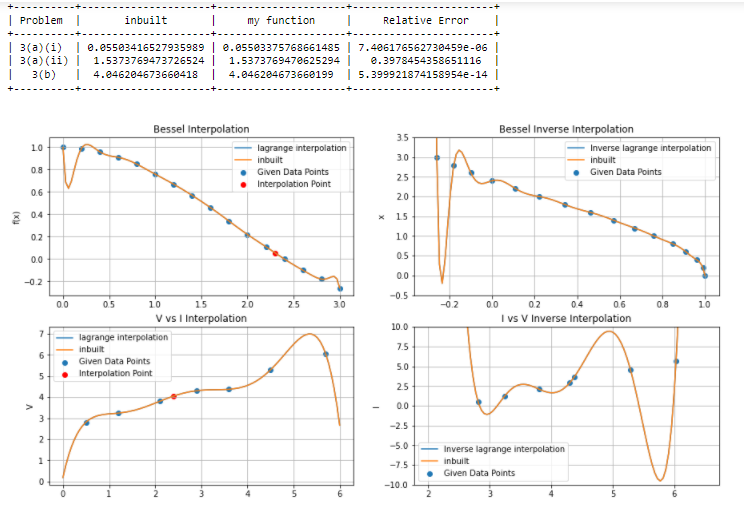
\includegraphics[width=15cm,height=12cm \textwidth]{Lagrange_Interpolation/Capture.PNG}
\caption{Lagrange Interpolation}
\end{figure}

%%%%%%%%%%%%%%%%%%%%%%%%%%%%%%%%%%%%%%%%%%%%%%%%%%%%%%%%%%%%%%%%%%%
\newpage
\begin{figure}[h]
    \centering
    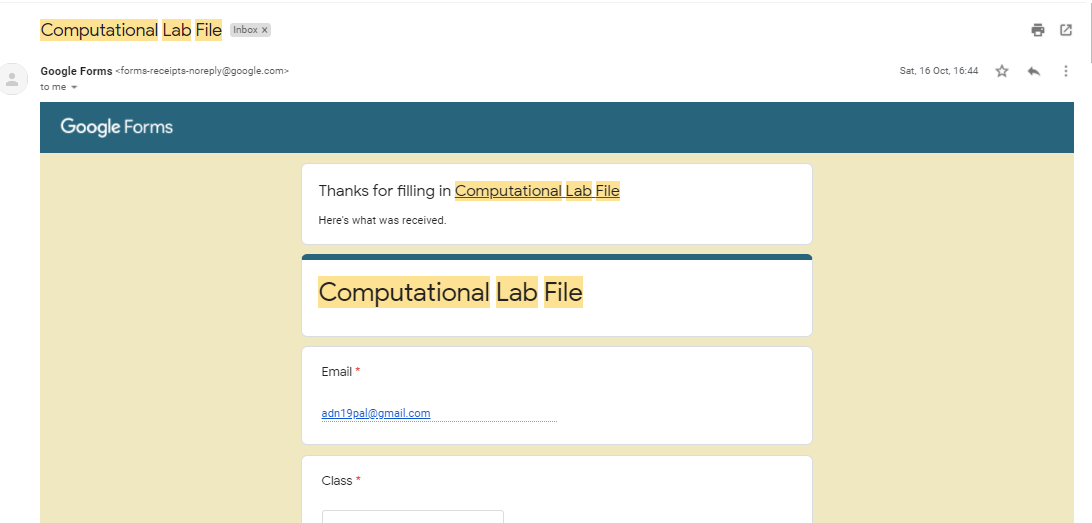
\includegraphics[width=14cm,height=12cm \textwidth]{4.PNG}
\caption{Radioactive Decay, RC Circuit and Stokes Law by Euler, RK2, RK4 Method}
\end{figure}
\section{Radioactive Decay, RC Circuit and Stokes Law by Euler, RK2, RK4 Method}
\lstinputlisting[language=python, 
caption=Radioactive Decay\text{,} RC Circuit and Stokes Law by Euler\text{,} RK2\text{,} and RK4 Method
]{Euler/euler.py}
\newpage
\clearpage
\begin{figure}[h]
    \centering
    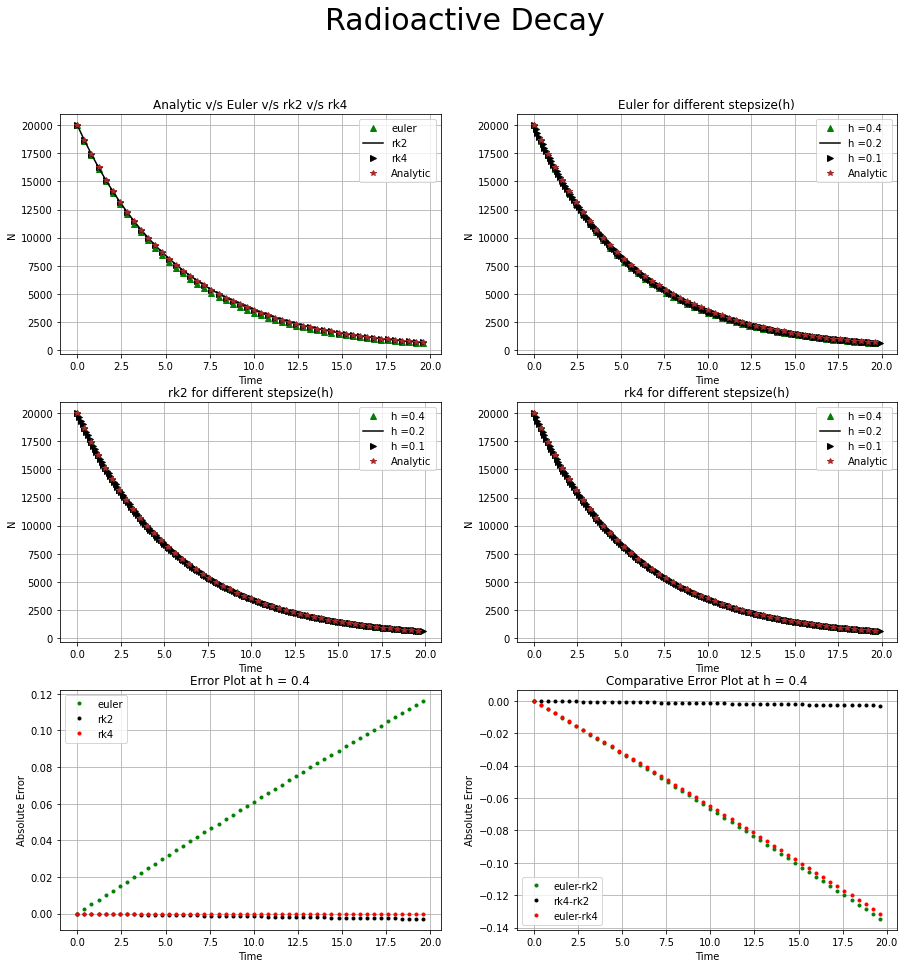
\includegraphics[width=14cm,height=12cm \textwidth]{Euler/radioactive.png}
\caption{Radioactive Decay}
\end{figure}
\newpage
\begin{figure}[h]
    \centering
    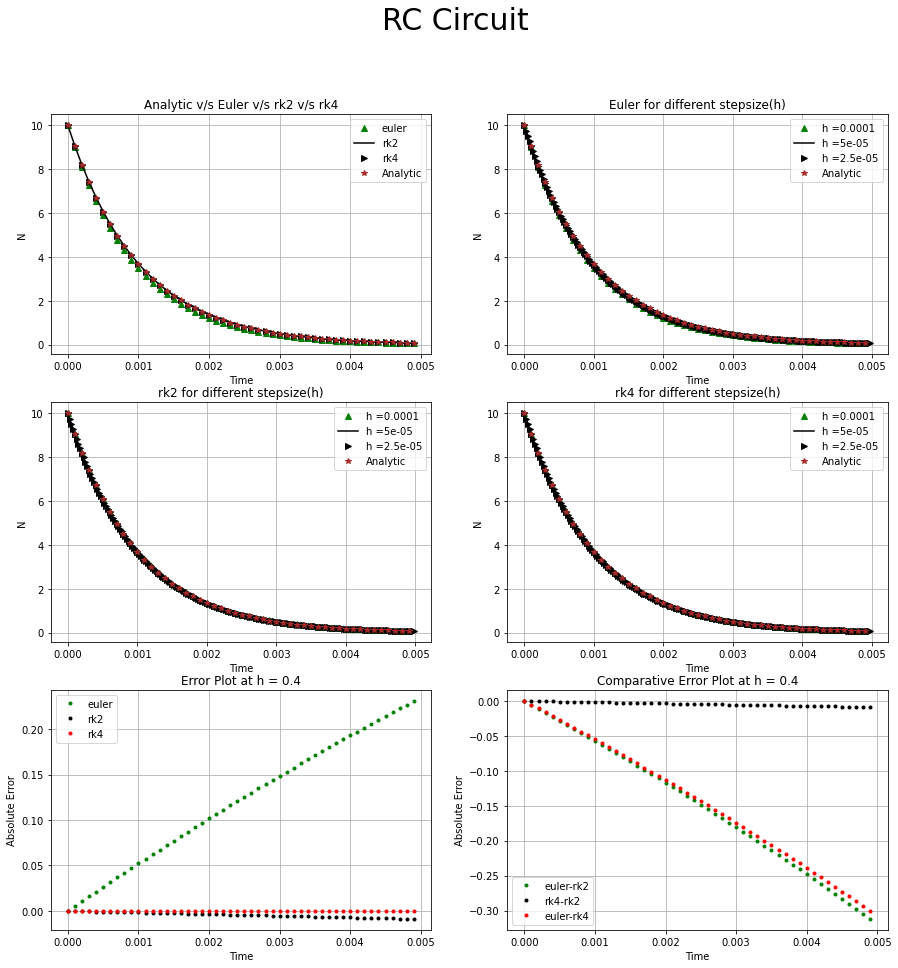
\includegraphics[width=14cm,height=12cm \textwidth]{Euler/rc.png}
\caption{RC Circuit}
\end{figure}
\newpage
\begin{figure}[h]
    \centering
    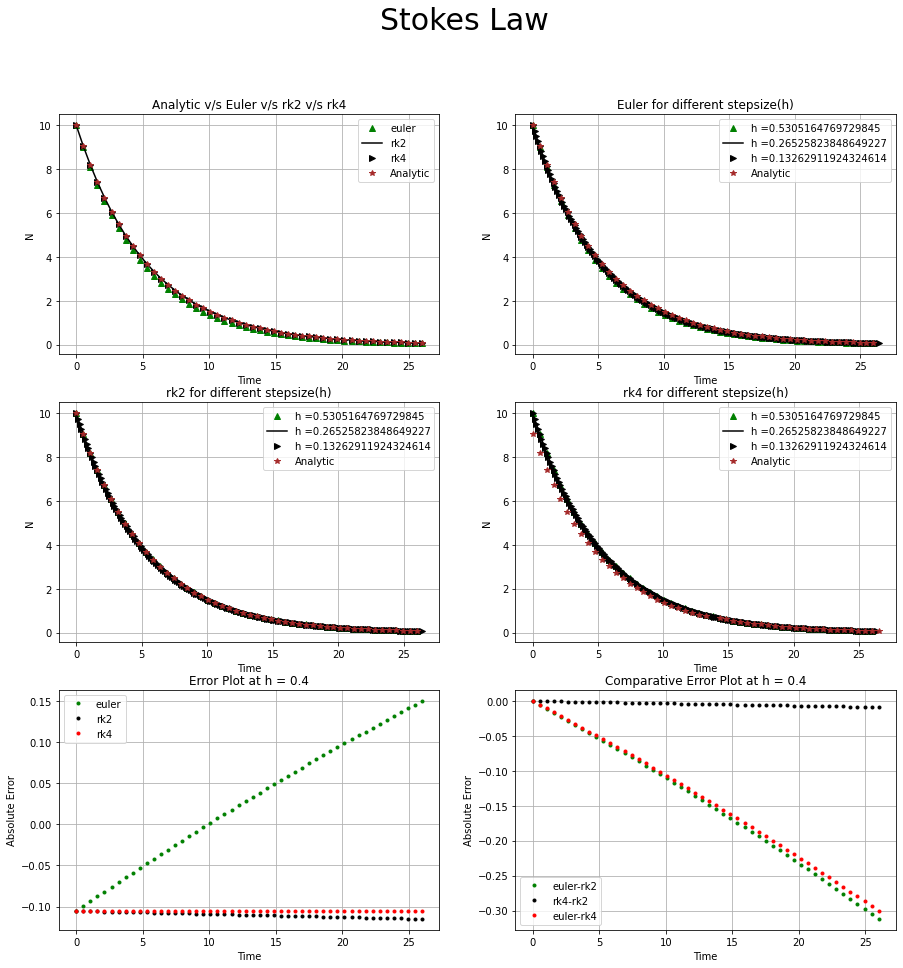
\includegraphics[width=14cm,height=12cm \textwidth]{Euler/stokes.png}
\caption{Stokes Law}
\end{figure}
%%%%%%%%%%%%%%%%%%%%%%%%%%%%%%%%%%%%%%%%%%%%%%%
\newpage
\begin{figure}[h]
    \centering
    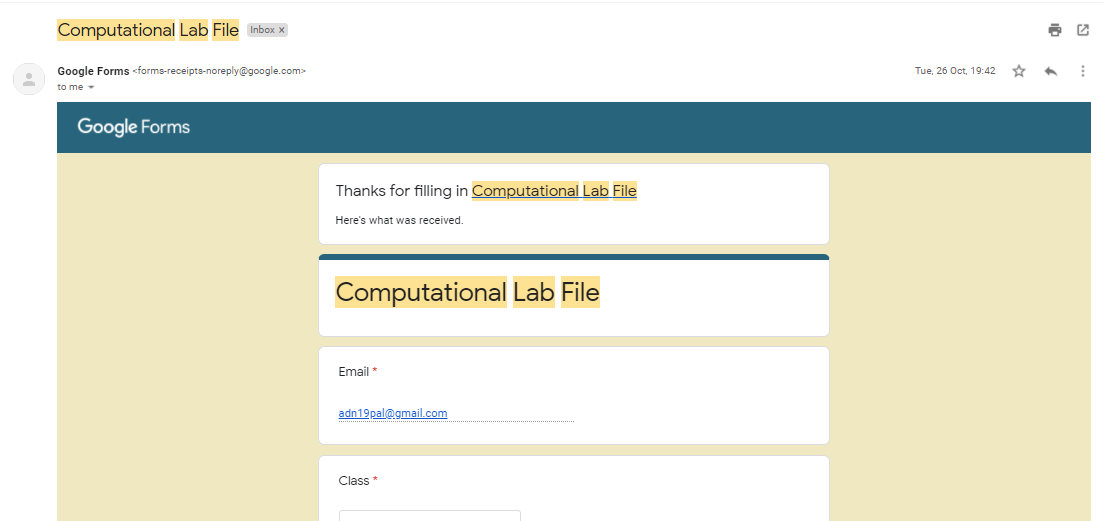
\includegraphics[width=15cm,height=13cm \textwidth]{5.PNG}
\caption{2nd Order Coupled diffential equations using Euler, RK2, RK4 Method}
\end{figure}
\section{2nd Order Coupled diffential equations using Euler, RK2, RK4 Method}
\lstinputlisting[language=python, 
caption=2nd Order coupled diffential equations using Euler\text{,} RK2 and RK4 Method
]{2nd_order_diff_using_rk2/rk2.py}

\clearpage
\begin{figure}[h]
    \centering
    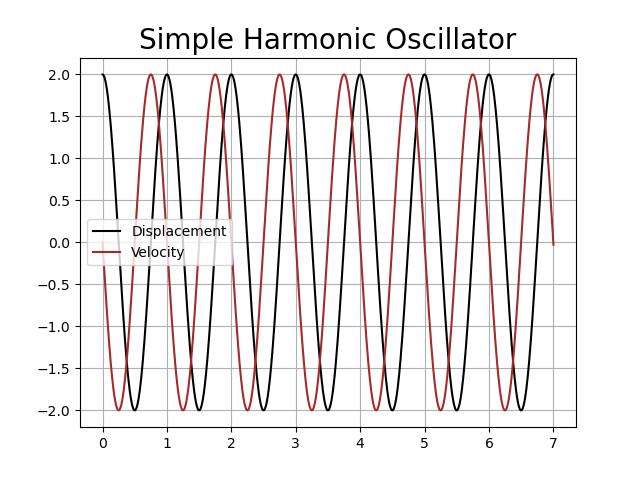
\includegraphics[width=15cm,height=13cm \textwidth]{2nd_order_diff_using_rk2/Figure_1.png}
\caption{Simple Harmonic Oscillator}
\end{figure}
\begin{figure}[h]
    \centering
    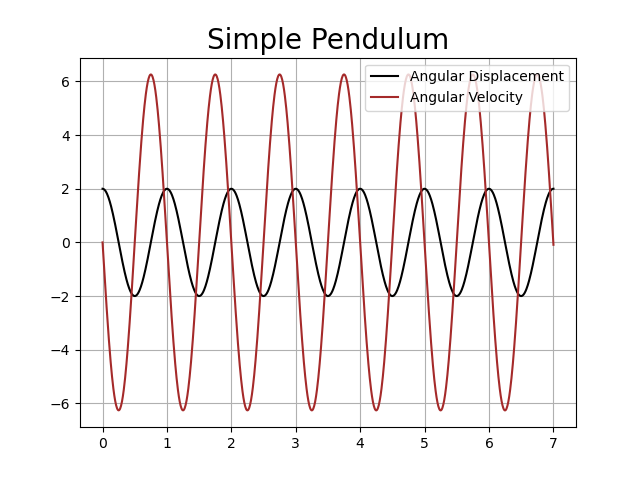
\includegraphics[width=15cm,height=13cm \textwidth]{2nd_order_diff_using_rk2/Figure_3.png}
\caption{Simple Pendulum}
\end{figure}
\newpage
\begin{figure}[h]
    \centering
    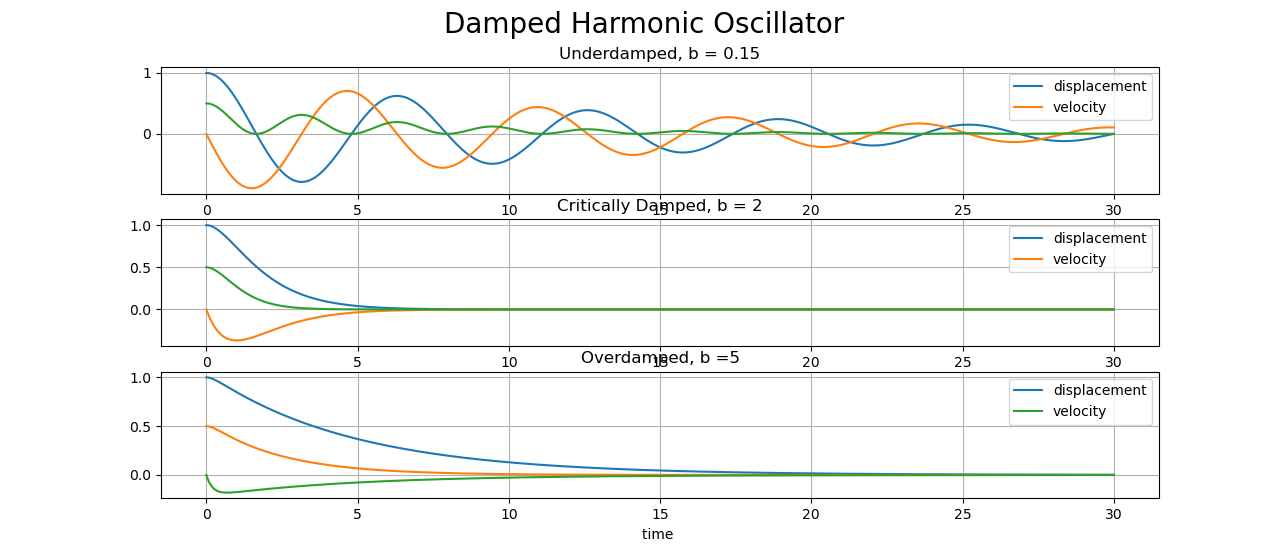
\includegraphics[width=15cm,height=13cm \textwidth]{2nd_order_diff_using_rk2/Figure_2.png}
\caption{Damped Harmonic Oscillator}
\end{figure}

%%%%%%%%%%%%%%%%%%%%%%%%%%%%%%%%%%%%%%%%%%%%%%%%%%%%%%%%%%%%%%%%%%%%%
\clearpage
\begin{figure}[h]
    \centering
    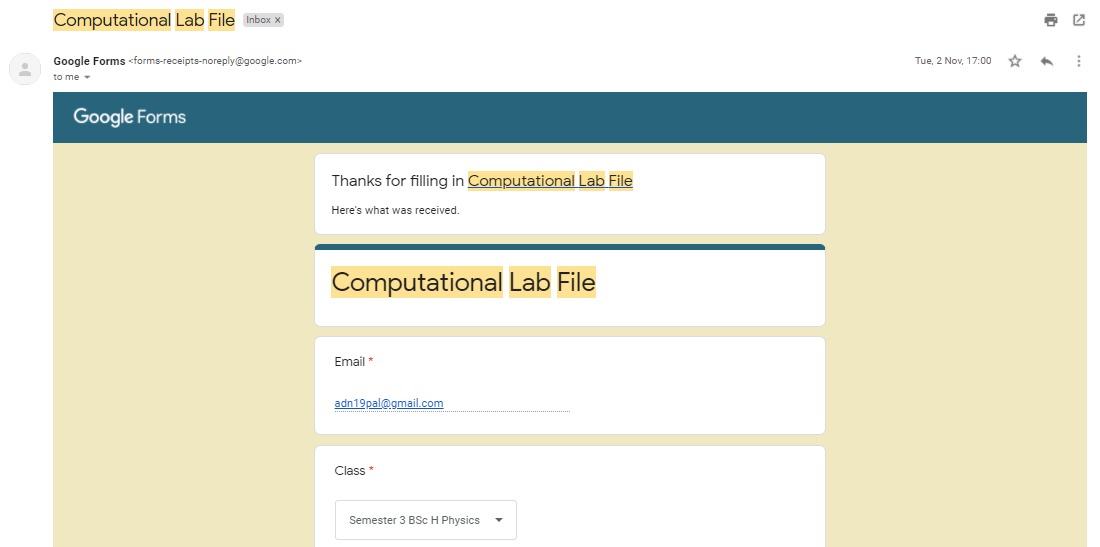
\includegraphics[width=14cm,height=12cm \textwidth]{6.PNG}
\caption{RK4 Method}
\end{figure}
\section{RK4 Method for Simulataneous Differential Equations}
\lstinputlisting[language=python, 
caption=RK4 Method for Simulataneous Differential Equations
]{rk4/rk4.py}

\newpage

\begin{figure}[h]
    \centering
    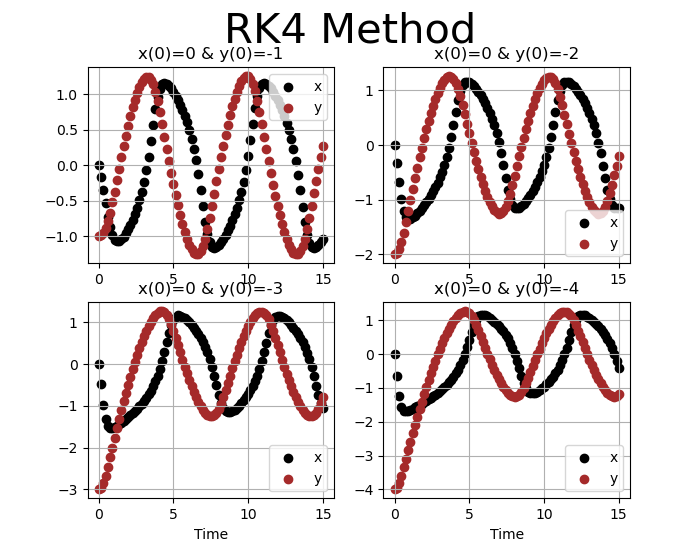
\includegraphics[width=14cm,height=12cm \textwidth]{rk4/Figure_1.png}
\caption{RK4 Method}
\end{figure}
\begin{figure}[h]
    \centering
    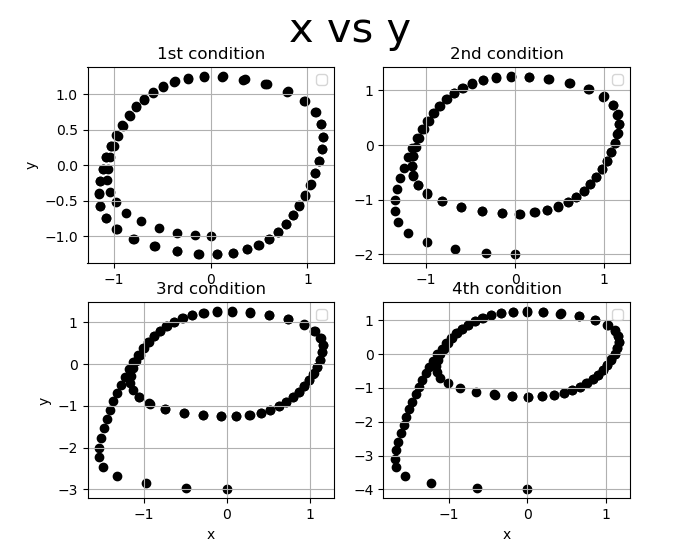
\includegraphics[width=14cm,height=12cm \textwidth]{rk4/Figure_2.png}
\caption{RK4 Method}
\end{figure}

%%%%%%%%%%%%%%%%%%%%%%%%%%%%%%%%%%%%%%%%%%%%%%%%%%%%%%%%%%%%%%%%%%%%%
\clearpage
\begin{figure}[h]
    \centering
    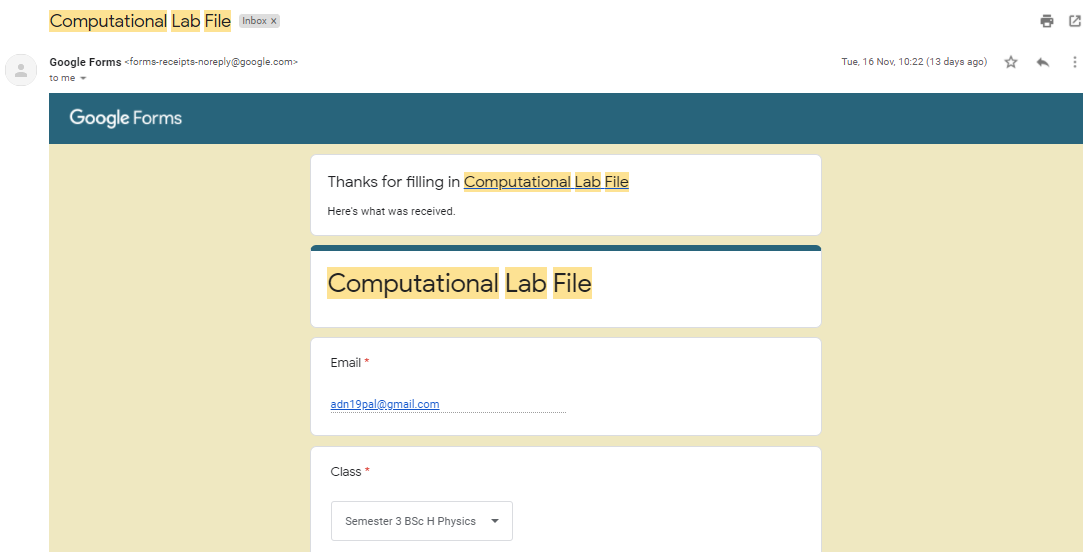
\includegraphics[width=14cm,height=5cm \textwidth]{7.PNG}
\caption{Gauss Elimination Method Output}
\end{figure}
\section{Gauss Elimination Method}
\lstinputlisting[language=python, 
caption=Gauss Elimination
]{Gauss_Elimination/gauss_elim.py}

\begin{figure}[h]
    \centering
    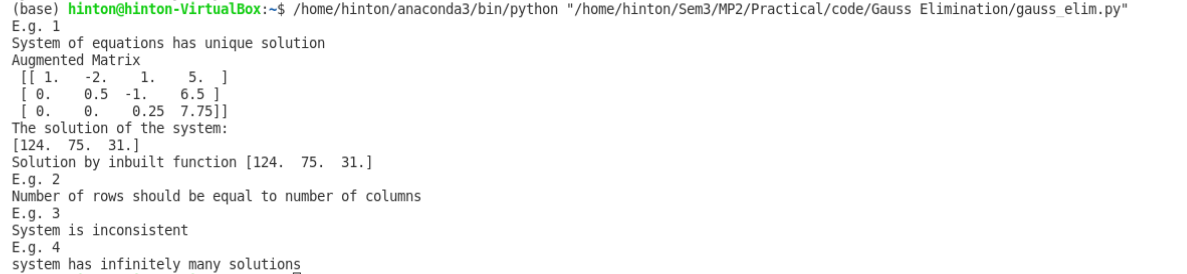
\includegraphics[width=14cm,height=5cm \textwidth]{Gauss_Elimination/Capture.PNG}
\caption{Gauss Elimination Method Output}
\end{figure}


%%%%%%%%%%%%%%%%%%%%%%%%%%%%%%%%%%%%%%%%%%%%%%%%%%%%%%%%%%%%%%%%%%%%%
\clearpage
\begin{figure}[h]
    \centering
    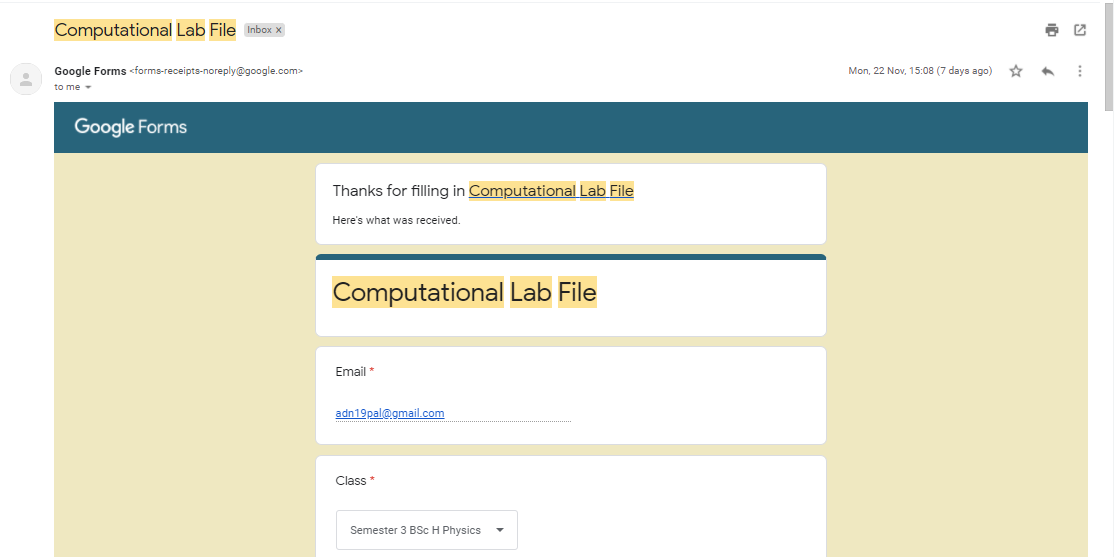
\includegraphics[width=15cm,height=8cm \textwidth]{8.PNG}
\caption{Gauss Seidel Method Output}
\end{figure}
\section{Gauss Seidel Method}
\lstinputlisting[language=python, 
caption=Gauss Seidel Method
]{Gauss_Seidel/gaussseidel.py}

\newpage
\begin{figure}[h]
    \centering
    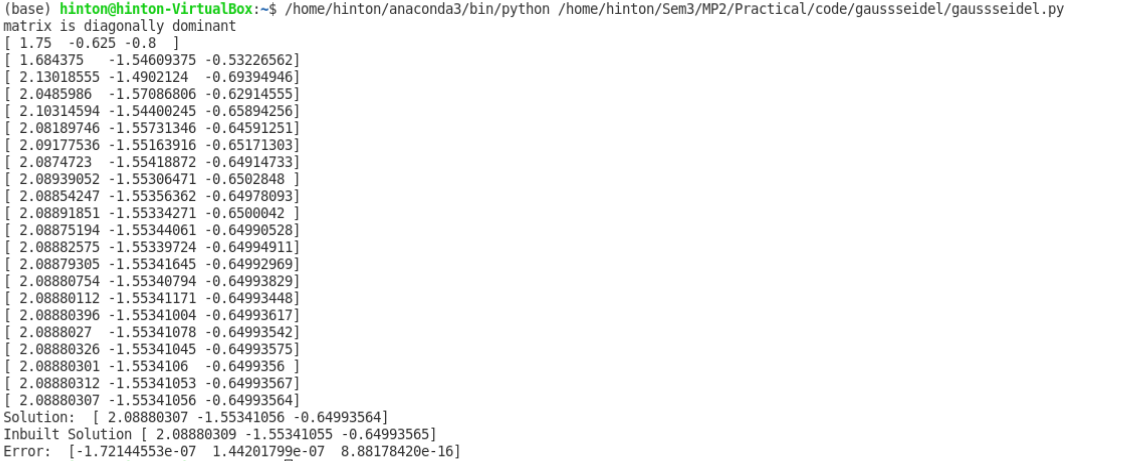
\includegraphics[width=15cm,height=8cm \textwidth]{Gauss_Seidel/Capture.PNG}
\caption{Gauss Seidel Method Output}
\end{figure}







\end{document}




